\section*{Team History \markright{HISTORY}}
\addcontentsline{toc}{section}{Team History}

Waterloo Rocketry \cite{waterloo-rocketry} is a student team representing the University of Waterloo (Ontario, Canada), in the 2025 Launch Canada Challenge (LC) \cite{launch-canada} with a high-altitude liquid bipropellant sounding rocket. 
The primary objective of the team is to provide students with 
%hands-on learning by tackling 
practical engineering challenges, 
while maintaining an atmosphere of learning and collaboration which is key to ensure team growth, continuity, and year-over-year competitiveness.
%Team growth and continuity hinge on maintaining an atmosphere of learning and collaboration, while remaining competitive and striving for year-to-year improvements. 
%Many past and present members have dedicated significant time and effort to the team, and continued success is a recognition of this commitment. 
Our continued success is a testament to the significant time past and present members have dedicated to the team, as well as the support and resources provided by the University of Waterloo, and the team's advisors
%, both from the University and industry, 
sharing valuable insights as the team develops more complex and sophisticated systems.

State estimation and control projects have been a topic of discussion on the team for the past decade. 
%The first serious research into active control began with the 2023 deployable payload project, whose intended scope consisted of an autonomous aerial vehicle which would be ejected from the rocket during descent, and autonomously navigate to the ground using an adjustable, inflatable wing. 
%This project proved to be too much scope for the payload team at the time, but led to significant research into the feasibility of state estimation. 
The payload that flew on the team's 2023 competition rocket, \emph{Leviathan of the Sky}, was essentially a state estimation prototype which relied on mostly existing avionics and sensors. % in order to minimize its scope. 
Due to both hardware and software issues the project produced no useful flight data, although the rocket launched successfully\footnote{The team achieved second place in the 30k SRAD hybrid/liquid class.} in the Intercollegiate Rocket Engineering Competition (IREC, at Spaceport America, New Mexico).

%In the aftermath of this failure 
It became clear that an independant payload
%which is largely defined by its independence from the rest of the rocket, 
was not a suitable platform for what the team wanted to work on, which was \emph{rocket} state estimation and control. 
Axial drag control surfaces, or ``airbrakes'', were relatively popular at IREC, due to accurate apogee being a large part of scoring. 
The team moved to the Launch Canada competition in 2024, and discussions with the organizers made flying active controls, including airbrakes and attitude control, seem feasible.
Conceptual designs for an airbrake system on the team's 2024 competition rocket, \emph{Borealis}, were drawn up shortly after the 2023 competition, and by the time the design cycle kicked off in fall it became clear that the scope of airbrakes warranted its own dedicated subsystem.
%and Controls was created to encompass dedicated active controls projects. 

There was considerable interest in the technical problems Controls was tackling, and the Controls team grew quickly to a similar size as the other rocket subsystems.
%and in just a few months, the Controls team grew to a similar size as many other rocket subsystems. 
Airbrakes were successfully integrated into and launched on Borealis in the LC 2025 competition\footnote{The team scored first, and became the first to fly a liquid bipropellant rocket in Canada.}.
However, with an apogee of less than 20k feet (due to under-filling of propellant), the rocket undershot the minimum target altitude for actuation of the airbrakes, and thus it was not possible to assess the control performance.

Due to the the difficulties in accurately controlling drag, and more long term team objectives, the decision was made that Controls would not attempt to fly airbrakes again, and instead the team is to develop a method for active roll control. 
Roll control is another proven technology in the amateur rocketry space. The two main justifications are stability of in-flight footage, and mitigation of roll-pitch coupling effects which are known to pose a significant risk to flight stability at higher altitudes, which the team is pursuing.

\section*{Aurora rocket\markright{AURORA}}
\addcontentsline{toc}{section}{Aurora rocket}
The Waterloo Rocketry team is developing the sounding rocket \emph{Aurora} for LC 2025.
Aurora is about 4.34m long with a diameter of 20.3cm, has a dry mass of about 51kg and carries about 35kg of propellants.
The liquid bipropellant engine is pressure-fed, and uses nitrous oxide as its oxidizer and ethanol as fuel.
The engine will burn for about 11s with a maximum thrust of about 10kN, which propels the rocket to about Mach 2.3 and a 16km apogee.
Next to the engine components and a parachute recovery system, Aurora carries scientific payloads -- and the experimental control system.

\begin{figure}[ht]
    \centering
    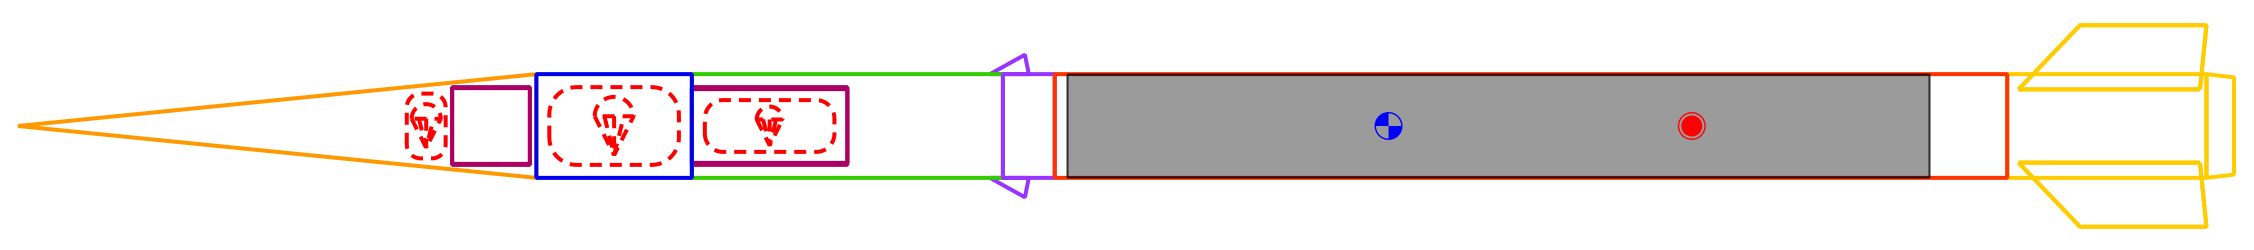
\includegraphics[width=0.9\linewidth]{images/introduction_aurora_OR.png}
    \caption[Aurora wireframe from OpenRocket]{Wireframe of the Aurora rocket. From OpenRocket, canards are shown in purple.}
    \label{fig:introduction_aurora}
\end{figure}

\subsubsection*{Canard roll control}
The rocket features an active control system in the form of controlled canards - small, steerable aerodynamic surfaces forward of the tail fins and center of mass.
These canards are designed to provide Aurora with roll control, the ability to stabilize the rocket around its longitudinal axis and to follow a roll program.
A low (or zero) roll rate inhibits \emph{coning}, a phenomena of coupled roll-pitch oscillations which drive an increasing precession of the rocket.
Excessive coning may end in the destruction of the rocket in flight.
Additionally, a controlled roll motion results in smoother pictures of the onboard cameras.

The successful development of a roll control system using canards may pave the way for a full attitude control system in the future, which should be able to reduce dispersion and increase performance of the next rocket.  

\section*{Development overview \markright{DEVELOPMENT}}
\addcontentsline{toc}{section}{Development Overview}
%\begin{itemize}
%    \item Simulation and design model have been developed independently to ensure that design can be validated with simulation 
%    \item who did what, other people involved (Tristan, Jacob), and outsourced work (Luca, Ben, Christine)
%    \item Rough timeline?
%\end{itemize}

%Finn designed the controller. Tristan and Jacob and I cheered him on.

The canards system can be roughly divided into four projects: actuation mechanics, the processor board and software, the motor control board, and the controller development/simulation -- this documentation deals with the latter.

The processor board is designed to interface with the onboard sensors and implement the control algorithms once they are designed.
The processor board hardware is largely unchanged from when it was originally developed for airbrakes, and the design of the canards version was completed through the end of December. The motor control board also had heritage to build on from airbrakes, and hardware for it was complete by the end of December.

Extensive firmware design for processor occurred in parallel with the hardware revision. 
%The embedded software has a modular architecture, so the controller and estimator tasks are implemented as modules.
The control design was done in Matlab, for embedded implementation this code is translated to C.
The decision was made to translate the code manually (instead of Matlab Coder), for the learning of the team members and to ease later troubleshooting.
%One module encapsulates the estimator’s mathematical operations, another the controller algorithm, while a minimal set of functions ensures the same input/output behavior as the original Simulink implementation. 
%The strategy for integrating and translating the estimator code from Matlab to C is to write a set of modules, one of which wraps the estimator math, and implement a minimum set of functions which provide the same input/output behaviour as the Simulink implementation. 
System validation is performed by a hardware-in-the-loop test, where the implementation of the control algorithms run live on the actual hardware while interacting with the simulation, and their outputs are checked against the full simulated loop.

The team has existing infrastructure for simulation, with the Flight Dynamics team relying primarily on OpenRocket, a proven rocket simulation software. 
Flight dynamics also serves as the primary systems engineering team, combining propulsion data to define the geometry and performance targets of the rocket. 
The simulation was developed in parallel with flight dynamics' own design phases.
Canard aerodynamics were developed jointly, with the Flight Dynamics team leading.

The simulation model and the actual controller design were researched and developed largely independently.
This ensures that the simulation serves as a valid testing platform for the control algorithms.

\subsubsection*{Simulation}
The Simulink plant model used for development is based on an existing canards project by Project Jupiter (University of São Paulo, Brazil). 
The model was largely rewritten in regards to aerodynamics, and new components were added to model sensor behaviour and to reflect actuator dynamics more accurately. 
In order to make team-wide integration easier, the simulation uses as much of the team's flight dynamics data as possible.

The model uses look-up tables for (varying) parameters like drag, thrust, and mass distribution, which are taken directly from the OpenRocket data for maximum parity. 
The model dynamics implemented in Simulink were validated by comparing the simulated trajectories of both Simulink and OpenRocket.

\subsubsection*{Controller design}

The control development was done using model-based design, as it is a proven and reliable method.
As the development was supposed to be as independent from simulation as possible, an effort was made to research and develop flight models from the ground up.
Rough rocket performance targets were available in October, from whose it was clear that control loop had to operate in a drastically varying environment (mainly very high velocity variations).

The decision to use LQR synthesis with a gain schedule for the controller, combined with an EKF for the state estimation was made early on.
LQR allowed a largely automatic controller design for the thousands of design points of the gain schedule.
The EKF was chosen to encompass the non-linear dynamics of rocket flight, and because it is a known approach in aerospace vehicle state estimation.
Both of these methods are completely dependent on the fidelity of their model, thus most of the control design effort has been developing these models.

Luckily, resources on aerospace vehicle dynamics and their control are readily available, in form of textbooks, an abundance of papers, and in lectures taken by the author.
Most of the model development was done by December, and focus shifted more on the controller and estimator algorithms. 
Common development and simulation was largely done in January, and tuning continued while embedded implementation started in February.
